\begin{ledgroupsized}[r]{120mm}
\footnotesize 
\pstart 
\noindent\textbf{\"{U}berlieferung:}
\pend
\end{ledgroupsized}
\begin{ledgroupsized}[r]{114mm}
\footnotesize 
\pstart \parindent -6mm
\makebox[6mm][l]{\textit{L}}%
Konzept: LH XXXVII 5 Bl. 120. 1 Bl. 2\textsuperscript{o}. 1 \unitfrac{1}{2} S. Wasserzeichen. Papier durch Erhaltungsma{\ss}nahmen gesichert.\\Cc 2, Nr. 00 \pend
\end{ledgroupsized}
%\normalsize
\vspace*{5mm}

\begin{ledgroup}
\footnotesize 
\pstart
\noindent\footnotesize{\textbf{Datierungsgr\"{u}nde}: 
Das Wasserzeichen im Textträger des vorliegenden Stücks ist für den Zeitraum vom Anfang 1674 bis zum Anfang 1675 belegt.}
\pend
\end{ledgroup}

\vspace*{8mm}
\pstart
\noindent
[120~r\textsuperscript{o}]
\pend
\pstart 
\normalsize
\centering De vi\protect\index{Sachverzeichnis}{vis} corporum per motum naturalem\protect\index{Sachverzeichnis}{motus naturalis} \edtext{continuatum}{\lemma{}\Bfootnote{continuatum \textit{erg. L}}} acquisita\\ Ratiocinatio
\pend 
\count\Afootins=1200
\count\Bfootins=1000
\pstart \vspace*{0.5em} 
\noindent Ponatur \edtext{globus \textit{A}}{\lemma{Ponatur}\Bfootnote{\textit{(1)} corpus a \textit{(2)} globus \textit{A} \textit{L}}} labi ex altitudine tanta \textit{ab} quanta sufficiat ad acquirendum impetum\protect\index{Sachverzeichnis}{impetus}, per quem \edtext{\textit{A}}{\lemma{quem}\Bfootnote{\textit{(1)} corpus labens \textit{(2)} \textit{a} \textit{(3)} \textit{A} \textit{L}}} superet \edtext{sphaeram \textit{B} sibi aequalem et aequiponderantem}{\lemma{superet}\Bfootnote{\textit{(1)} corpus sibi aequale et aequiponderans \textit{B} idque \textit{(2)} sphaeram \textit{B} \textit{(a)} similem sibi \textit{(b)} sibi aequalem et aequiponderantem \textit{L}}} \edtext{tanto virium\protect\index{Sachverzeichnis}{vis} excessu ut eam elevare possit}{\lemma{}\Bfootnote{tanto virium\protect\index{Sachverzeichnis}{vis} excessu \textit{(1)} eamque \textit{(2)} ut eam elevare possit \textit{erg.} \textit{L}}} elevet per tantam altitudinem quanta est ipsius sphaerae seu ex \textit{d} \edtext{in \textit{c}. Quod fiet si sphaera labens ex \textit{a} in \textit{b}, impingat in eminentiam \textit{eF} prodeuntem ex chorda \textit{cgh} circa trochleam \textit{g} replicata sphaeramque \textit{B} sustinente. Sed ponamus debere}{\lemma{in \textit{c}.}\Bfootnote{\textit{(1)} Porro numerus sphaerarum \textit{(2)} Sed ad restituenda omnia in statum priorem, \textit{(a)} opus esset \textit{(b)} deberet \textit{(3)} Quod fiet [...] ponamus debere \textit{L}}} elevare integram columnam \edtext{talium}{\lemma{}\Bfootnote{talium \textit{erg.} \textit{L}}} sphaerarum, in recta linea \textit{ab} collocabilium.
\pend
\pstart
Harum sphaerarum numerum appellemus \edtext{$\alpha$}{\lemma{appellemus}\Bfootnote{\textit{(1)} \textit{a} \textit{(2)} $\upsilon$ \textit{(3)} $\xi$ \textit{(4)} $\alpha$ \textit{L}}}. 
\pend
\pstart
Ergo \textit{A} labens ex altitudine \textit{ab} elevabit 1.
\pend 
\pstart
Duplicetur altitudo \textit{ab} erit duplicata altitudo \edtext{l\edtext{apsus\protect\index{Sachverzeichnis}{lapsus} \textit{ae}}{\lemma{lapsus}\Bfootnote{\textit{(1)}\ $a$ \textit{(2)}\ \textit{ae} \textit{L}}}}{\lemma{}\Afootnote{\textit{Über} lapsus $ae$: cum debeat $\alpha$\vspace{-8mm}}} duplicabitur quoque numerus sphaerarum \edtext{elevandarum}{\lemma{}\Bfootnote{elevandarum \textit{erg.} \textit{L}}}. At vero \edtext{quadruplicabuntur vires seu numerus}{\lemma{vero}\Bfootnote{\textit{(1)} quadruplicabitur numerus virium \textit{(2)} quadruplicabuntur vires seu numerus \textit{L}}} sphaerarum elevabilium. Et multiplicata altitudine semper magis multiplicabuntur vires\protect\index{Sachverzeichnis}{vis} quam onus, si quidem vera sunt quae hactenus ab omnibus fere recipiuntur quod scilicet \edtext{gravium impetus crescant}{\lemma{scilicet}\Bfootnote{\textit{(1)} gravia crescant \textit{(2)} gravium impetus crescant \textit{L}}} in duplicata altitudinum ratione. Ergo denique superabitur onus a viribus\protect\index{Sachverzeichnis}{vis}, ac proinde assumta altitudine sufficienti, \edtext{sequetur plena machinae restitutio}{\lemma{sufficienti,}\Bfootnote{\textit{(1)} sequi omnimodam plenam machinae restitutionem\protect\index{Sachverzeichnis}{machinae restitutio|textit} \textit{(2)} sequetur plena machinae restitutio \textit{L}}}, quae altitudo an in praxi haberi possit nihil refert ad institutum, sufficit demonstrari posse, aut restitutionem perfectam\protect\index{Sachverzeichnis}{restitutio perfecta} ex natura motus sequi, aut ejus proportiones\protect\index{Sachverzeichnis}{proportio} receptas exactas non esse. Quod credere malim. \setline{6}Calculus hic erit:
\pend
\count\Afootins=1200
\count\Bfootins=1200
\pstart
\vspace*{1em}
\noindent
\begin{tabular}{ccccll}
$A$ 
{labens\renewcommand*{\raggedleftmarginnote}{} \reversemarginpar\marginnote{\scriptsize\hspace{46mm}10}}
ex &elevabit in altitudinem sui&cum debeat elevare&&&\\
altitudine&sphaeras&sphaeras&id est e.g.&&\\
1&1&$\alpha$ 1&10&9&8\\
2&4&$\alpha$ 2&20&18&16\\
3&9&$\alpha$ 3&30&27&24\\
{4\renewcommand*{\raggedleftmarginnote}{}\reversemarginpar\marginnote{\scriptsize\hspace{46mm}15}}
&16&$\alpha$ 4&40&36&32\\
5&25&$\alpha$ 5&50&45&40\\
6&36&$\alpha$ 6&60&54&48\\
7&49&$\alpha$ 7&70&63&65\\
8&\uline{64}&$\alpha$ 8&80&72&\uuline{64}\\
{9\renewcommand*{\raggedleftmarginnote}{}\reversemarginpar\marginnote{\scriptsize\hspace{46mm}20}}
&\uline{81}&$\alpha$ 9&90&\uuline{81}&72\\
10&\uline{100}&$\alpha$ 10&\uuline{100}&90&80\\
\end{tabular}
%\begin{tabular}{ccccll}
%$A$ labens ex &elevabit in altitudinem sui&cum debeat elevare&&&\\
%altitudine&sphaeras&sphaeras&id est e.g.&&\\
%1&1&$\alpha$ 1&10&9&8\\
%2&4&$\alpha$ 2&20&18&16\\
%3&9&$\alpha$ 3&30&27&24\\
%4&16&$\alpha$ 4&40&36&32\\
%5&25&$\alpha$ 5&50&45&40\\
%6&36&$\alpha$ 6&60&54&48\\
%7&49&$\alpha$ 7&70&63&65\\
%8&\uline{64}&$\alpha$ 8&80&72&\uuline{64}\\
%9&\uline{81}&$\alpha$ 9&90&\uuline{81}&72\\
%10&\uline{100}&$\alpha$ 10&\uuline{100}&90&80\\
%\end{tabular}
\pend
\pstart
\vspace*{1em}
Si \setline{22}ergo numerus [$\alpha$]\edtext{}{\Bfootnote{a\textit{\ L \"{a}ndert Hrsg.}}} ponatur esse 10. decuplicanda est altitudo prima. Si \edtext{9.}{\lemma{Si}\Bfootnote{\textit{(1)} novem \textit{(2)} 9. \textit{L}}}, noncuplicanda. Et generaliter posito incremento\protect\index{Sachverzeichnis}{incrementum} impetus\protect\index{Sachverzeichnis}{impetus} in duplicata ratione spatiorum \edtext{si multiplicetur}{\lemma{si}\Bfootnote{\textit{(1)} multiplicanda est \textit{(2)} multiplicetur \textit{L}}} altitudo 1. per numerum sphaerarum [$\alpha$]\edtext{}{\Bfootnote{a\textit{\ L \"{a}ndert Hrsg.}}}. Sequetur restitutio perfecta\protect\index{Sachverzeichnis}{restitutio perfecta}; \edtext{ex hypothesi recepta}{\lemma{perfecta;}\Bfootnote{\textit{(1)} ex vulgari hypothesi \textit{(2)} ex hypothesi recepta \textit{L}}} incrementi\protect\index{Sachverzeichnis}{incrementum}. Instituenda hic experimenta\protect\index{Sachverzeichnis}{experimentum}: (1) ex qua altitudine labens corpus datum possit elevare aliud datum sibi aequale, inaequale, aequiponderans, \edtext{aut non\hfill aequiponderans}{\lemma{}\Bfootnote{aut non aequiponderans \textit{erg. L}}},\hfill simile\hfill dissimile,\hfill possit\hfill elevare\hfill in\hfill \textso{altitudinem quantam}.
\pend
\pstart\noindent
\centering
%\begin{wrapfigure}[24]{l}{0.45\textwidth} 
%\vspace{-4mm}
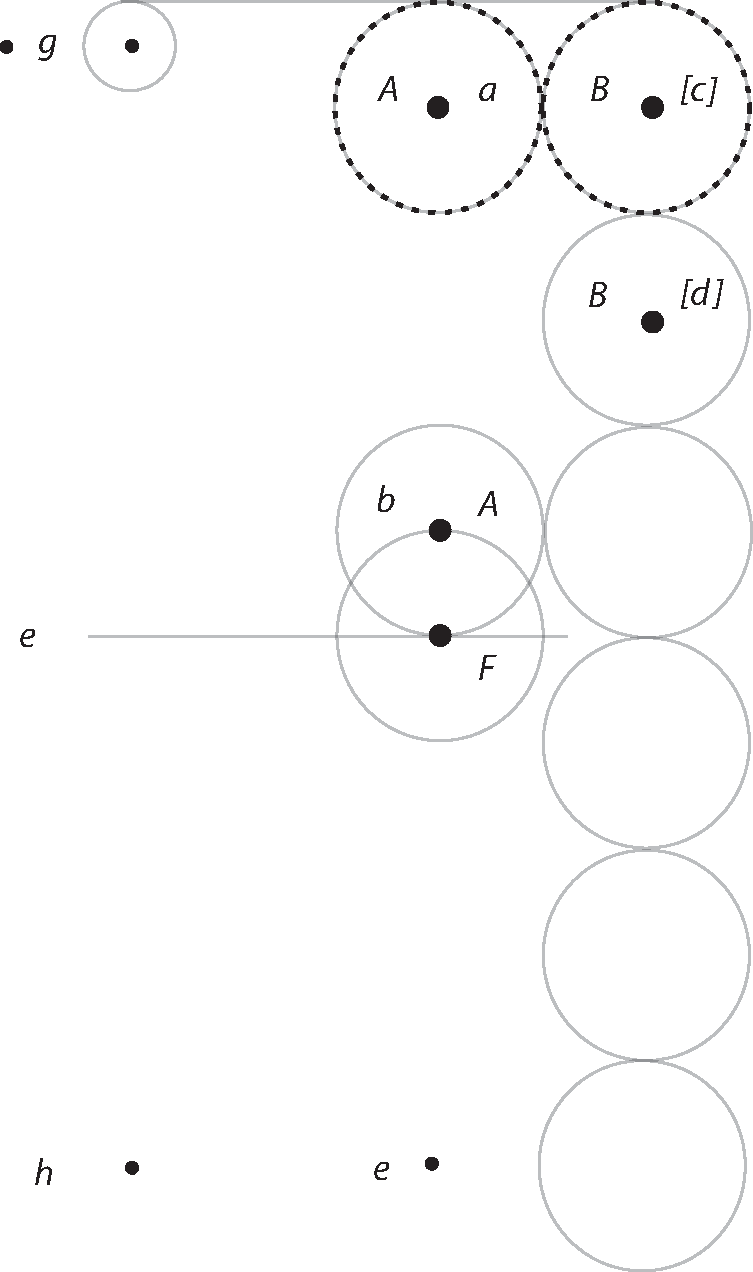
\includegraphics[trim = 0mm -5mm 0mm 0mm, clip, width=0.45\textwidth]{images/lh03705_120r-d1.pdf}\\
%\vspace{0.5em}
             \noindent \centering [\textit{Fig. 1, tlw. Blindzeichnung}] 
%\end{wrapfigure}
\pend
\vspace{1em}
\pstart\noindent Certum \setline{1}est enim corpus labens ex quantulacunque altitudine elevare posse aequiponderans quiescens, sed \edtext{}{\lemma{}\Bfootnote{sed \textbar\ et \textit{gestr.} \textbar\ in \textit{L}}}in altitudinem exiguam.\\
(2) Experiendum quanta altitudine opus sit, ut corpus parvum labens levet corpus magnum sensibiliter in altitudinem quantulamcumque.
\\
(3) Quamdiu duret impetus\protect\index{Sachverzeichnis}{impetus} post concursum seu quamdiu corpus unum alteri ob lapsum praeponderet, quod alioqui non praeponderaret.
\\
(4) Quanta sit resistentia aeris\protect\index{Sachverzeichnis}{resistentia aeris} et an aeris resistentia\protect\index{Sachverzeichnis}{resistentia aeris} crescat cum descensu.
\\
(5) An non incrementum\protect\index{Sachverzeichnis}{incrementum} gravium sit continue decrescens, quod mihi probare posse videor ac sphaera labens elevabit integram columnam sphaerarum sibi aequalium per totam lapsus\protect\index{Sachverzeichnis}{lapsus} altitudinem dispositarum, atque ita ipsa labens subintrabit in locum ultimae, summa autem labi incipiet sequeturque machinae restitutio\protect\index{Sachverzeichnis}{restitutio machinae} in statum priori per omnia similem, aut necesse est doctrinam receptam de incremento\protect\index{Sachverzeichnis}{incrementum} motus gravium\protect\index{Sachverzeichnis}{motus gravium} non satis firmo fundamento niti progressionemque ejus esse non uniformem, sed ut mihi \edtext{probabile videtur decrescentem}{\lemma{mihi}\Bfootnote{\textit{(1)} videtur decrescentem \textit{(2)} probabile videtur decrescentem \textit{L}}}. [120~v\textsuperscript{o}]\\
(6) An \edtext{corpus majus}{\lemma{An}\Bfootnote{\textit{(1)} ex quanto \textit{(2)} majore \textit{(3)} corpus m \textit{(4)} corpus majus \textit{L}}} ex minore, majore, an eadem altitudine lapsum elevet corpus sibi aequiponderans et aequale in altitudinem corporis sui, quam corpus minus elevat aliud \edtext{sibi aequiponderans}{\lemma{}\Bfootnote{sibi aequiponderans \textit{erg.} \textit{L}}} minus. Meretur hoc inprimis observari ducet enim nos in intimas impetus\protect\index{Sachverzeichnis}{impetus} hujus proportiones\protect\index{Sachverzeichnis}{proportio}.
\pend
\pstart 
Sunto duo corpora \edtext{homogenea}{\lemma{}\Bfootnote{homogenea \textit{erg. L}}} aequiponderantia et aequalia gravia et magna. Sunto duo alia levia et parva. Quaestio est an utrobique eadem altitudine lapsus\protect\index{Sachverzeichnis}{lapsus} opus sit, ut labens elevet quiescens in altitudinem corporis sui, aut in altitudinem datam; an \edtext{potius}{\lemma{an}\Bfootnote{\textit{(1)} non \textit{(2)} potius \textit{L}}} majore opus sit, \edtext{aut an}{\lemma{sit,}\Bfootnote{\textit{(1)} an vero \textit{(2)} aut an \textit{L}}} minore, et qua proportione\protect\index{Sachverzeichnis}{proportio}.
\pend
%\newpage
\pstart 
(7) An resistentia corporum\protect\index{Sachverzeichnis}{resistentia corporum} \edtext{lapsum excipientium}{\lemma{}\Bfootnote{lapsum excipientium \textit{erg.} \textit{L}}} crescat ut vis\protect\index{Sachverzeichnis}{vis} labentium. Pone corpus $a$ \edtext{impingens}{\lemma{$a$}\Bfootnote{\textit{(1)} labens \textit{(2)} impingens \textit{L}}} in $b$ \edtext{aequiponderans aut praeponderans}{\lemma{}\Bfootnote{aequiponderans aut praeponderans \textit{erg.} \textit{L}}} id superare per \edtext{aliquod}{\lemma{per}\Bfootnote{\textit{(1)} datum \textit{(2)} aliquod \textit{L}}} temporis spatium, donec impetus\protect\index{Sachverzeichnis}{impetus} evanescat, et $b$ restituat se in aequiponderationem, aut praeponderationem, quaeritur an durante isto temporis spatio impetus\protect\index{Sachverzeichnis}{impetus} impingentis decresceat seu evanescere incipiat uniformiter, an difformiter et qua proportione. Et an ipsum corpus resistens magis resistat momento\protect\index{Sachverzeichnis}{momentum} aliquo sequente quam antecedente.
\pend
\pstart 
Sed hic examinandum esset quid aeris resistentia\protect\index{Sachverzeichnis}{resistentia aeris} conferat an ipsa quoque cum impetu\protect\index{Sachverzeichnis}{impetus} lapsus\protect\index{Sachverzeichnis}{lapsus} \edtext{labentis}{\lemma{}\Bfootnote{labentis \textit{erg. L}}} crescat.
\pend
\pstart 
Ante omnia autem experiendum est quanta altitudine lapsus\protect\index{Sachverzeichnis}{lapsus} opus habeat corpus, ad elevandum aliud aequiponderans in altitudinem corporis. Et quae sit ratio altitudinis lapsus\protect\index{Sachverzeichnis}{lapsus}. Si corpora aequiponderantia sunt magna, aut non magna quidem, gravia tamen magis; ad altitudinem lapsu minorum.
\pend
\pstart  
Quibus aliisque quae nunc enumerare prolixum foret constitutis doctrina motuslapsus\protect\index{Sachverzeichnis}{doctrina motus gravium} gravium\protect\index{Sachverzeichnis}{motus gravium} in majore luce constituetur.
\pend
\count\Afootins=1500
\count\Bfootins=1500
